\section{Field Study} % (fold)
\label{sec:field_study}

The the end of the project we tested the visualization directly in school in two different sessions to test the two different target groups and applications: In one class the teacher used \HG to explain the conferences at the end and after World War II and in another class one week later the students used \HG in the computer room to inform themselves about the Bipolar World 1945-1993 and prepare an overview. We are presenting the planning, conduction and results of the two studies.


\subsection{Usage as Teaching Material} % (fold)
\label{sub:usage_as_teaching_material}

Our research question for the first test was if \HG is suitable as a teaching material in the classroom. The teacher wanted to use the software to explain the historical context (name, time and location), the content and the consequences of four major conferences at the end of World War II: Casablanca and Tehran 1943, Yalta and Potsdam 1945.

\subsubsection{Planning} % (fold)
\label{ssub:planning-1}

We had the following research hypotheses:
\begin{enumerate}
  \item Effectiveness $H_{efs-1.1}$: \HG is well suited to impart the historical context (What?, When?, Where?, How?) of an historical event.
  \item Effectiveness $H_{efs-1.2}$: \HG is not suited to impart the historical coherences (Why?) of historical events.
  \item Satisfaction $H_{sat-1.1}$:  The teacher will have no technical oder usability problem while presenting the topic with \textsc{HistoGlobe}.
  \item Satisfaction $H_{sat-1.2}$:  The students will appreciate the visualization of the topic with \textsc{HistoGlobe}.
\end{enumerate}

Because there is just one test in one class with one teacher and the course of a history class is somewhat arbitrary, we did not use any quantitative measures to test our research hypotheses. We also could not measure any efficiency, which is usually important for usability testing. Out main focus is finding out whether the current concept of \HG is suited as a teaching material and if there are any usability flaws. We decided to use the following methods:

\begin{enumerate}
  \item Video recording of the whole class to analyze the usage of the teacher afterwards.
  \item Semi-structural interview with the teacher after the class to get more insight into his usage of the software.
  \item Short Questionnaire (see: appendix \ref{ssub:questionnaires}) for the students after the class.
\end{enumerate}

% subsubsection planning (end)

\subsection{Conduction} % (fold)
\label{sub:conduction-1}
On Thursday, 16.04.2015 from 11:35 until 13:05 the teacher held a lesson about the four major conferences after World War II. In 15 minutes during the lesson he actively used \HG planned to show the students the location, the date, the name and an image of the conference. He asked the students about the context and content of the conferences using the visualization. He swapped between his own prepared teaching slides and \HG. He once used the software spontaneously (see Figure \ref{fig:teacher}): A student asked ``What is a satellite state?'', the teacher zoomed out of the map, so that Eastern Europe is visible and explained the Soviet satellite sates (GDR, Poland, Czechoslovakia, ...).

\begin{figure}[ht]
  \begin{center}
    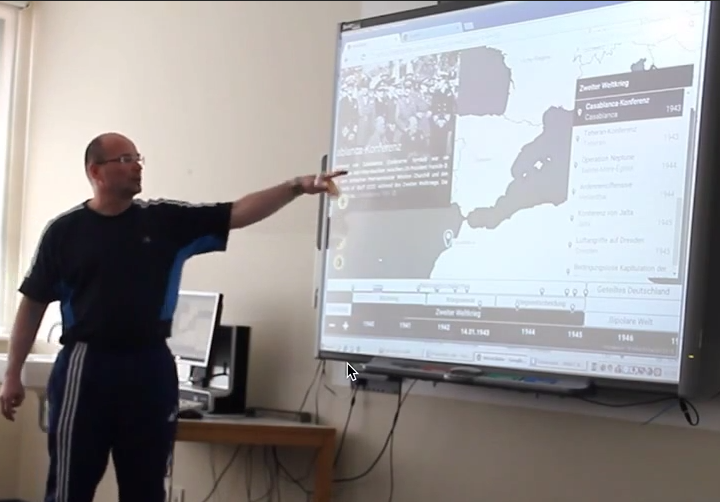
\includegraphics[width=0.4\textwidth]{graphics/teacher-2.png}
    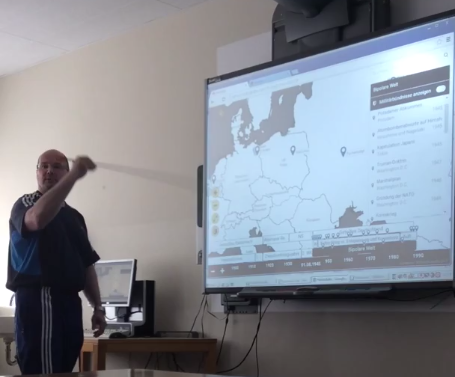
\includegraphics[width=0.4\textwidth]{graphics/teacher-1.png}
  \end{center}
  \caption{The usage of \HG as a teaching material in the classroom}
  \label{fig:teacher}
\end{figure}

% subsection conduction (end)

\subsection{Results} % (fold)
\label{sub:results-1}

While the teacher used \HG we noticed the following:

\begin{itemize}
  \item The visualization was only in the HighContrast. It seemed suitable for the very bright lighting condition.
  \item The teacher used only the mouse, not the Smartboard, as an input device.
  \item The Hivent List was the only element to select an Hivent, but not the Timeline or the Map.
  \item Sometimes there are labels of minor countries on the map, but the important ones are missing. The label display concept has to be thought through again.
  \item The current date of the visualization is barely visible and should be more prominent.
\end{itemize}

In the interview with the teacher after the lesson we revealed the following important results of the field study:

\begin{itemize}
  \item The big advantage of \HG is the map, especially navigation and zooming.
  \item The teacher sees great potential in visualizing territorial development of countries and membership to alliances.
  \item \HG is suited for him to show the name, date and location of an Hivent, but not the coherences. In his opinion this shall also not be the focus of the development.
  \item He believes that the effect on the students are only minor, because they are used to work with a Smartboard and \HG does not give them extra information \\[0.8em]
  $\Rightarrow$ He concludes that \HG is only partially useful as a teaching material but he believes it was much more helpful for students to learn.
\end{itemize}

The students gave us a good insight into the effect on their understanding from the questionnaire (Figure \ref{fig:studyresults-1}):

\begin{itemize}
  \item The satisfaction with the subject history in general seems to be close to a normal distribution.
  \item Most students found \HG interesting, became curious about the software and are willing to work more with \HG
  \item The biggest advantages seem to be the summary and the overview that the visualization gives to them. Also the factor of time and the picturing of the Hivents because of the images seem well-made.
  \item Most students did not appreciate the black-and-white design of the HighContrast mode and were confused by the visualization. Some students complained that \HG was not used enough in class in order to understand and appreciate it more.
\end{itemize}

\begin{figure}[ht]
  \begin{center}
    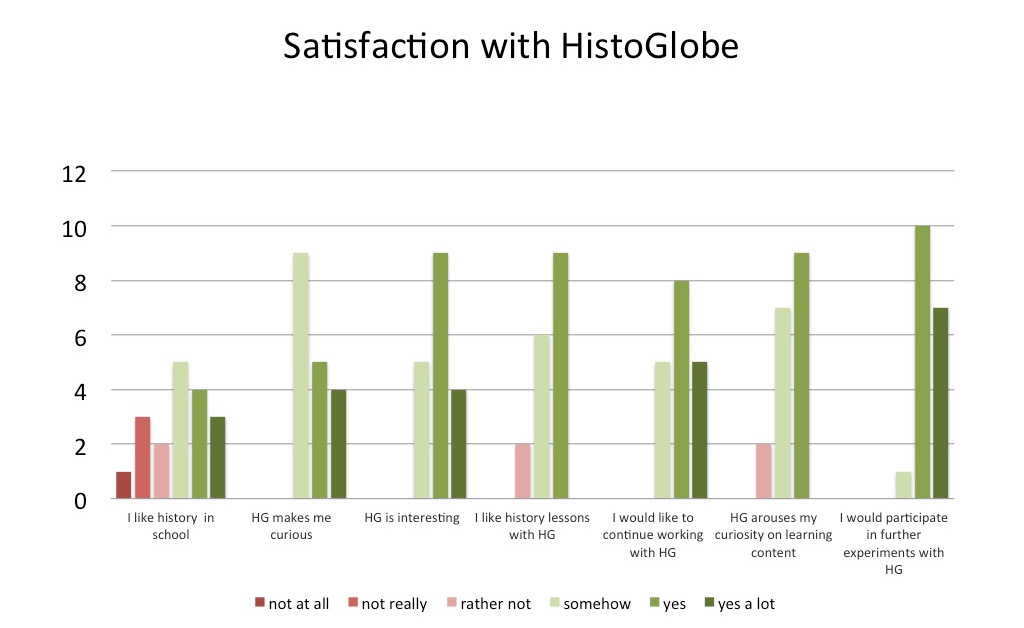
\includegraphics[width=0.9\textwidth]{graphics/test-1-satisfaction.jpg} \\[0.5em]
    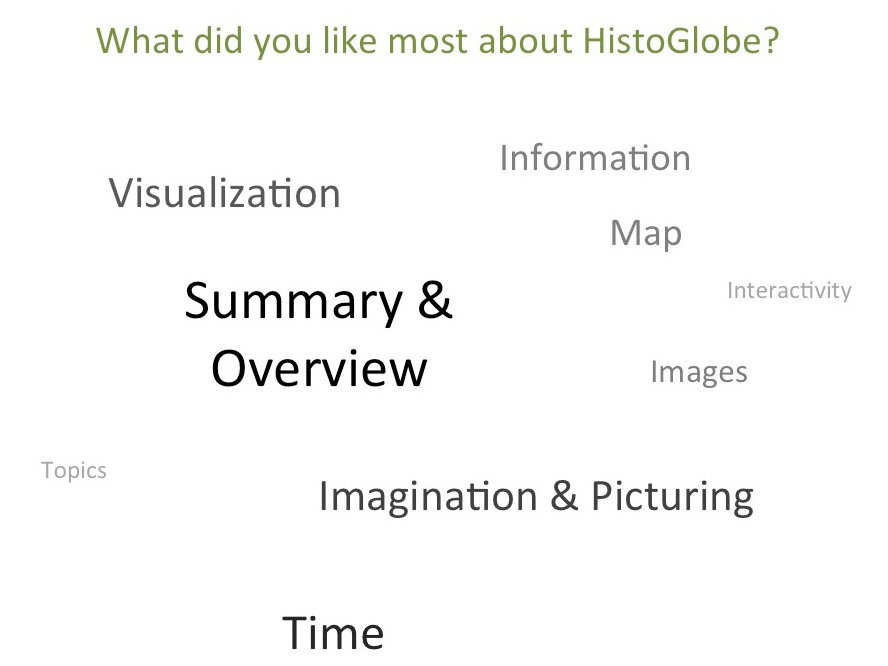
\includegraphics[width=0.45\textwidth]{graphics/test-1-tagcloud-pos.jpg}
    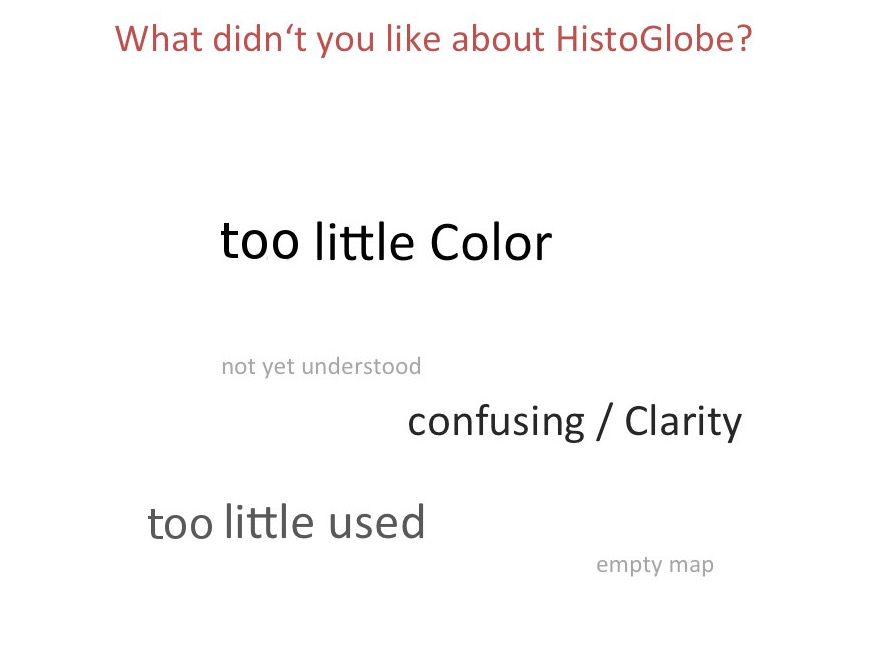
\includegraphics[width=0.45\textwidth]{graphics/test-1-tagcloud-neg.jpg}
  \end{center}
  \caption{Results of the first field study with students}
  \label{fig:studyresults-1}
\end{figure}

Finally, we see potential evidence for accepting our research hypotheses. It seems to be that \HG is well suited to impart the \textit{What?, When?, Where?} and \textit{How?} of an Hivent ($H_{efs-1.1}$) but not at all for the explanation of the \textit{Why?}: historical coherences ($H_{efs-1.2}$). From our observation, hypothesis $H_{sat-1.1}$ seems to hold and also $H_{sat-1.1}$ is also likely due to the results from the questionnaire. It has to mentioned that this analysis is neither exhaustive nor statistically accurate, because we have not conducted a classical user study.

% subsection results (end)
% subsection usage_as_teaching_material (end)


\subsection{Usage as Study Material} % (fold)
\label{sub:usage_as_study_material}

One week after the first field study we had a second one in a computer pool of Lobdeburgschule. The students had the task to research about events in the cold and the hot phases of the Bipolar World 1945-1993. The output was supposed to be a timeline with an overview about the development in the Bipolar World.

\subsubsection{Planning} % (fold)
\label{ssub:planning-2}

We had the following research hypotheses:
\begin{enumerate}
  \item Effectiveness $H_{efs-2.1}$: \HG is well suited to understand the historical context (What?, When?, Where?, How?) of an historical event.
  \item Effectiveness $H_{efs-2.2}$: \HG is not suited to understand the historical coherences (Why?) of historical events.
  \item Satisfaction $H_{sat-2.1}$: The students will have no technical oder usability problems while doing research with \textsc{HistoGlobe}.
\end{enumerate}

In the same way as in the first field study we used no quantitative but only qualitative methods to evaluate our hypotheses. We observed the students while working, asked specific questions and used the same questionnaire as the week before to measure a difference between the usage of \HG for teaching and for learning purposes.

% subsubsection planning (end)

\subsubsection{Conduction} % (fold)
\label{ssub:conduction-2}
On Friday, 22.04.2015, from 11:35 until 13:05 the students performed the task stated above. We used the 75 minutes in which the students were supposed to fulfill the task to find out about the usage of \HG and the advantages, disadvantages and problems with the software.

\begin{figure}[tb]
  \begin{center}
    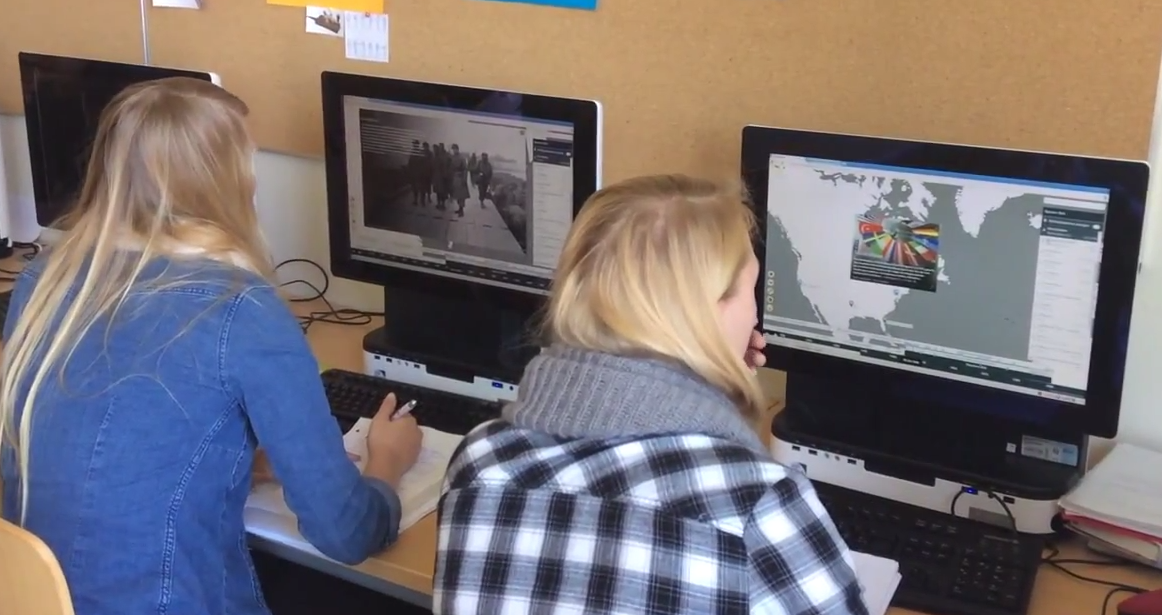
\includegraphics[width=0.45\textwidth]{graphics/students-1.png}
    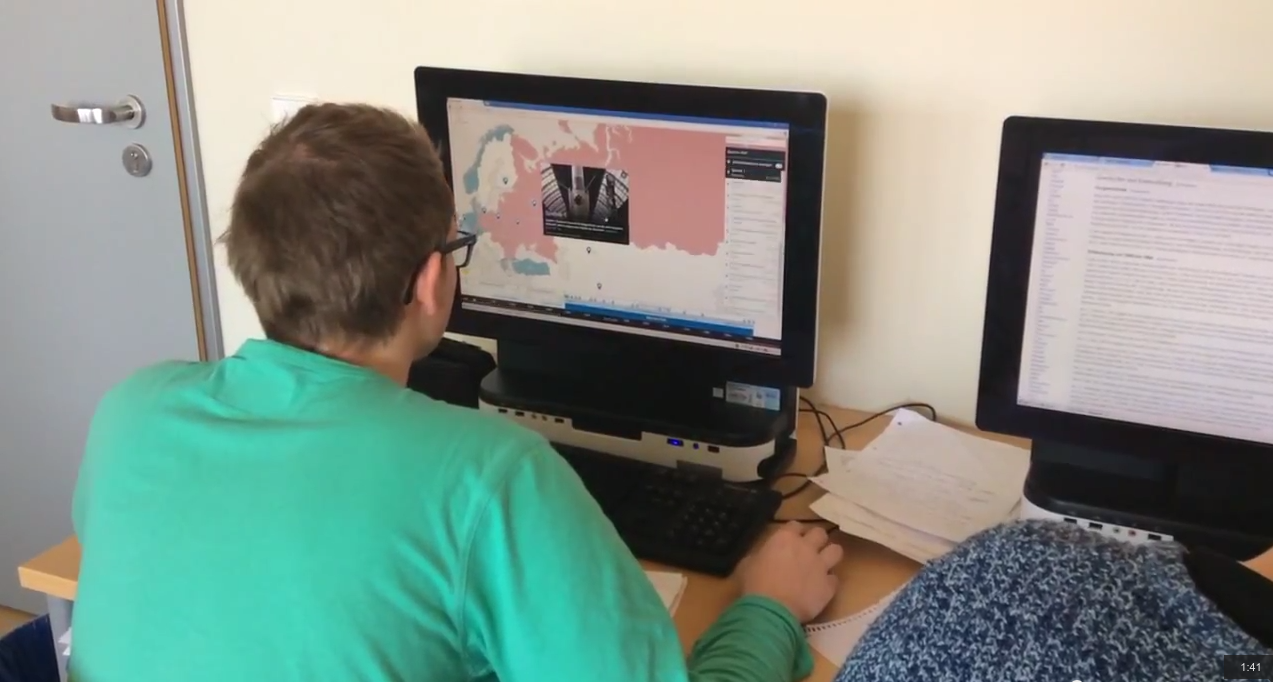
\includegraphics[width=0.45\textwidth]{graphics/students-2.png}
    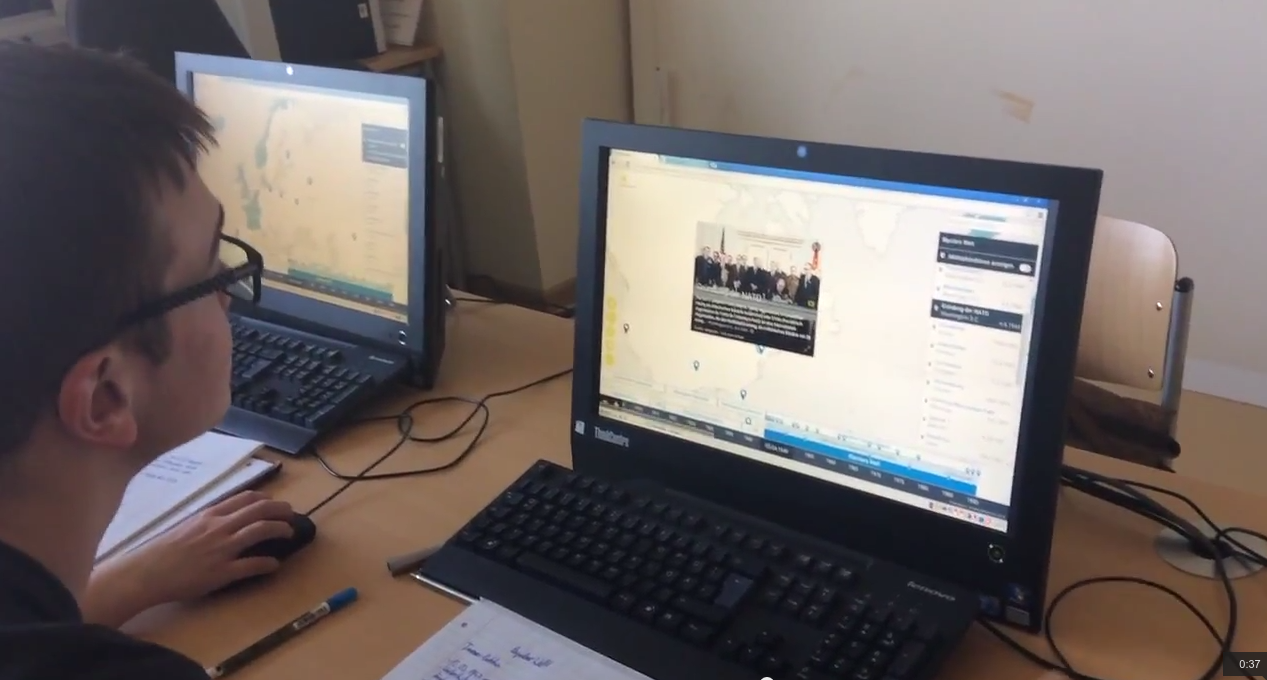
\includegraphics[width=0.45\textwidth]{graphics/students-3.png}
    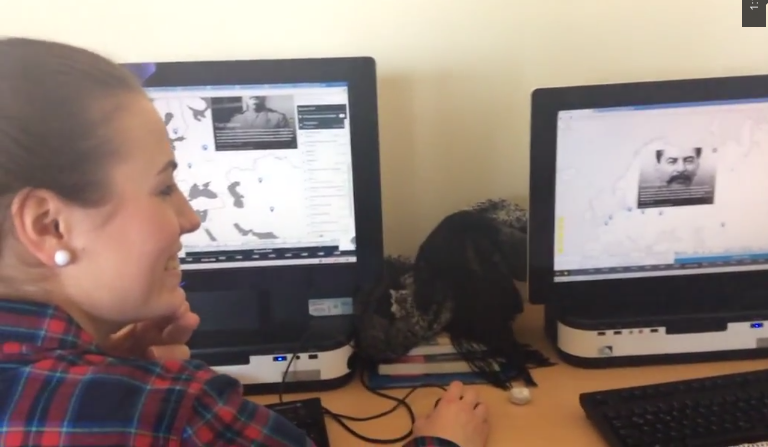
\includegraphics[width=0.45\textwidth]{graphics/students-4.png}
  \end{center}
  \caption{The usage of \HG as a learning material for the students}
  \label{fig:students}
\end{figure}

% subsubsection conduction (end)

\subsubsection{Results} % (fold)
\label{ssub:results-2}

% subsubsection results (end)
% subsection usage_as_study_material (end)
% section field_study (end)
